%%%%%%%%%%%%%%%%%%%% author.tex %%%%%%%%%%%%%%%%%%%%%%%%%%%%%%%%%%%
%
% sample root file for your "contribution" to a contributed volume
%
% Use this file as a template for your own input.
%
%%%%%%%%%%%%%%%% Springer %%%%%%%%%%%%%%%%%%%%%%%%%%%%%%%%%%


% RECOMMENDED %%%%%%%%%%%%%%%%%%%%%%%%%%%%%%%%%%%%%%%%%%%%%%%%%%%
\documentclass[graybox]{svmult}

% choose options for [] as required from the list
% in the Reference Guide

\usepackage{mathptmx}       % selects Times Roman as basic font
\usepackage{helvet}         % selects Helvetica as sans-serif font
\usepackage{courier}        % selects Courier as typewriter font
\usepackage{type1cm}        % activate if the above 3 fonts are
                            % not available on your system
%
\usepackage{makeidx}         % allows index generation
\usepackage{graphicx}        % standard LaTeX graphics tool
                             % when including figure files
\usepackage{multicol}        % used for the two-column index
\usepackage[bottom]{footmisc}% places footnotes at page bottom

% see the list of further useful packages
% in the Reference Guide

\makeindex             % used for the subject index
                       % please use the style svind.ist with
                       % your makeindex program

%%%%%%%%%%%%%%%%%%%%%%%%%%%%%%%%%%%%%%%%%%%%%%%%%%%%%%%%%%%%%%%%%%%%%%%%%%%%%%%%%%%%%%%%%

\begin{document}

\title*{Contribution Title}
% Use \titlerunning{Short Title} for an abbreviated version of
% your contribution title if the original one is too long
\author{Name of First Author and Name of Second Author}
% Use \authorrunning{Short Title} for an abbreviated version of
% your contribution title if the original one is too long
\institute{Name of First Author \at Name, Address of Institute, \email{name@email.address}
\and Name of Second Author \at Name, Address of Institute \email{name@email.address}}
%
% Use the package "url.sty" to avoid
% problems with special characters
% used in your e-mail or web address
%
\maketitle

\abstract*{Each chapter should be preceded by an abstract (10--15 lines long) that summarizes the content. The abstract will appear \textit{online} at \url{www.SpringerLink.com} and be available with unrestricted access. This allows unregistered users to read the abstract as a teaser for the complete chapter. As a general rule the abstracts will not appear in the printed version of your book unless it is the style of your particular book or that of the series to which your book belongs.
Please use the 'starred' version of the new Springer \texttt{abstract} command for typesetting the text of the online abstracts (cf. source file of this chapter template \texttt{abstract}) and include them with the source files of your manuscript. Use the plain \texttt{abstract} command if the abstract is also to appear in the printed version of the book.}

\abstract{Each chapter should be preceded by an abstract (10--15 lines long) that summarizes the content. The abstract will appear \textit{online} at \url{www.SpringerLink.com} and be available with unrestricted access. This allows unregistered users to read the abstract as a teaser for the complete chapter. As a general rule the abstracts will not appear in the printed version of your book unless it is the style of your particular book or that of the series to which your book belongs.\newline\indent
Please use the 'starred' version of the new Springer \texttt{abstract} command for typesetting the text of the online abstracts (cf. source file of this chapter template \texttt{abstract}) and include them with the source files of your manuscript. Use the plain \texttt{abstract} command if the abstract is also to appear in the printed version of the book.}

\section{Section Heading}
\label{sec:1}
Use the template \emph{chapter.tex} together with the Springer document class SVMono (monograph-type books) or SVMult (edited books) to style the various elements of your chapter content in the Springer layout.

Instead of simply listing headings of different levels we recommend to
let every heading be followed by at least a short passage of text.
Further on please use the \LaTeX\ automatism for all your
cross-references and citations. And please note that the first line of
text that follows a heading is not indented, whereas the first lines of
all subsequent paragraphs are.

\section{Section Heading}
\label{sec:2}
% Always give a unique label
% and use \ref{<label>} for cross-references
% and \cite{<label>} for bibliographic references
% use \sectionmark{}
% to alter or adjust the section heading in the running head
Instead of simply listing headings of different levels we recommend to
let every heading be followed by at least a short passage of text.
Further on please use the \LaTeX\ automatism for all your
cross-references and citations.

Please note that the first line of text that follows a heading is not indented, whereas the first lines of all subsequent paragraphs are.

Use the standard \verb|equation| environment to typeset your equations, e.g.
%
\begin{equation}
a \times b = c\;,
\end{equation}
%
however, for multiline equations we recommend to use the \verb|eqnarray| environment\footnote{In physics texts please activate the class option \texttt{vecphys} to depict your vectors in \textbf{\itshape boldface-italic} type - as is customary for a wide range of physical subjects}.
\begin{eqnarray}
a \times b = c \nonumber\\
\vec{a} \cdot \vec{b}=\vec{c}
\label{eq:01}
\end{eqnarray}

\subsection{Subsection Heading}
\label{subsec:2}
Instead of simply listing headings of different levels we recommend to
let every heading be followed by at least a short passage of text.
Further on please use the \LaTeX\ automatism for all your
cross-references\index{cross-references} and citations\index{citations}
as has already been described in Sect.~\ref{sec:2}.

\begin{quotation}
Please do not use quotation marks when quoting texts! Simply use the \verb|quotation| environment -- it will automatically render Springer's preferred layout.
\end{quotation}


\subsubsection{Subsubsection Heading}
Instead of simply listing headings of different levels we recommend to
let every heading be followed by at least a short passage of text.
Further on please use the \LaTeX\ automatism for all your
cross-references and citations as has already been described in
Sect.~\ref{subsec:2}, see also Fig.~\ref{fig:1}\footnote{If you copy
text passages, figures, or tables from other works, you must obtain
\textit{permission} from the copyright holder (usually the original
publisher). Please enclose the signed permission with the manuscript. The
sources\index{permission to print} must be acknowledged either in the
captions, as footnotes or in a separate section of the book.}

Please note that the first line of text that follows a heading is not indented, whereas the first lines of all subsequent paragraphs are.

% For figures use
%
\begin{figure}[b]
\sidecaption
% Use the relevant command for your figure-insertion program
% to insert the figure file.
% For example, with the graphicx style use
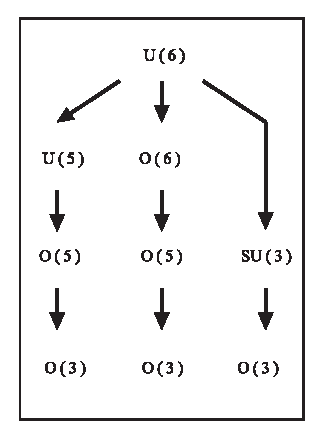
\includegraphics[scale=.65]{figure}
%
% If no graphics program available, insert a blank space i.e. use
%\picplace{5cm}{2cm} % Give the correct figure height and width in cm
%
\caption{If the width of the figure is less than 7.8 cm use the \texttt{sidecapion} command to flush the caption on the left side of the page. If the figure is positioned at the top of the page, align the sidecaption with the top of the figure -- to achieve this you simply need to use the optional argument \texttt{[t]} with the \texttt{sidecaption} command}
\label{fig:1}       % Give a unique label
\end{figure}


\paragraph{Paragraph Heading} %
Instead of simply listing headings of different levels we recommend to
let every heading be followed by at least a short passage of text.
Further on please use the \LaTeX\ automatism for all your
cross-references and citations as has already been described in
Sect.~\ref{sec:2}.

Please note that the first line of text that follows a heading is not indented, whereas the first lines of all subsequent paragraphs are.

For typesetting numbered lists we recommend to use the \verb|enumerate| environment -- it will automatically render Springer's preferred layout.

\begin{enumerate}
\item{Livelihood and survival mobility are oftentimes coutcomes of uneven socioeconomic development.}
\begin{enumerate}
\item{Livelihood and survival mobility are oftentimes coutcomes of uneven socioeconomic development.}
\item{Livelihood and survival mobility are oftentimes coutcomes of uneven socioeconomic development.}
\end{enumerate}
\item{Livelihood and survival mobility are oftentimes coutcomes of uneven socioeconomic development.}
\end{enumerate}


\subparagraph{Subparagraph Heading} In order to avoid simply listing headings of different levels we recommend to let every heading be followed by at least a short passage of text. Use the \LaTeX\ automatism for all your cross-references and citations as has already been described in Sect.~\ref{sec:2}, see also Fig.~\ref{fig:2}.

For unnumbered list we recommend to use the \verb|itemize| environment -- it will automatically render Springer's preferred layout.

\begin{itemize}
\item{Livelihood and survival mobility are oftentimes coutcomes of uneven socioeconomic development, cf. Table~\ref{tab:1}.}
\begin{itemize}
\item{Livelihood and survival mobility are oftentimes coutcomes of uneven socioeconomic development.}
\item{Livelihood and survival mobility are oftentimes coutcomes of uneven socioeconomic development.}
\end{itemize}
\item{Livelihood and survival mobility are oftentimes coutcomes of uneven socioeconomic development.}
\end{itemize}

\begin{figure}[t]
\sidecaption[t]
% Use the relevant command for your figure-insertion program
% to insert the figure file.
% For example, with the option graphics use
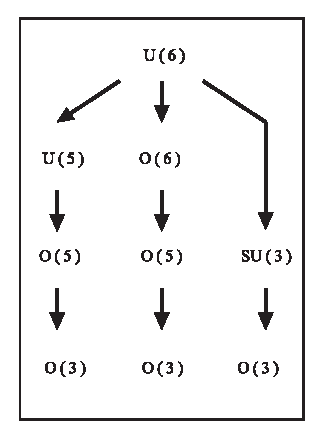
\includegraphics[scale=.65]{figure}
%
% If no graphics program available, insert a blank space i.e. use
%\picplace{5cm}{2cm} % Give the correct figure height and width in cm
%
%\caption{Please write your figure caption here}
\caption{If the width of the figure is less than 7.8 cm use the \texttt{sidecapion} command to flush the caption on the left side of the page. If the figure is positioned at the top of the page, align the sidecaption with the top of the figure -- to achieve this you simply need to use the optional argument \texttt{[t]} with the \texttt{sidecaption} command}
\label{fig:2}       % Give a unique label
\end{figure}

\runinhead{Run-in Heading Boldface Version} Use the \LaTeX\ automatism for all your cross-references and citations as has already been described in Sect.~\ref{sec:2}.

\subruninhead{Run-in Heading Italic Version} Use the \LaTeX\ automatism for all your cross-refer\-ences and citations as has already been described in Sect.~\ref{sec:2}\index{paragraph}.
% Use the \index{} command to code your index words
%
% For tables use
%
\begin{table}
\caption{Please write your table caption here}
\label{tab:1}       % Give a unique label
%
% Follow this input for your own table layout
%
\begin{tabular}{p{2cm}p{2.4cm}p{2cm}p{4.9cm}}
\hline\noalign{\smallskip}
Classes & Subclass & Length & Action Mechanism  \\
\noalign{\smallskip}\svhline\noalign{\smallskip}
Translation & mRNA$^a$  & 22 (19--25) & Translation repression, mRNA cleavage\\
Translation & mRNA cleavage & 21 & mRNA cleavage\\
Translation & mRNA  & 21--22 & mRNA cleavage\\
Translation & mRNA  & 24--26 & Histone and DNA Modification\\
\noalign{\smallskip}\hline\noalign{\smallskip}
\end{tabular}
$^a$ Table foot note (with superscript)
\end{table}
%
\section{Section Heading}
\label{sec:3}
% Always give a unique label
% and use \ref{<label>} for cross-references
% and \cite{<label>} for bibliographic references
% use \sectionmark{}
% to alter or adjust the section heading in the running head
Instead of simply listing headings of different levels we recommend to
let every heading be followed by at least a short passage of text.
Further on please use the \LaTeX\ automatism for all your
cross-references and citations as has already been described in
Sect.~\ref{sec:2}.

Please note that the first line of text that follows a heading is not indented, whereas the first lines of all subsequent paragraphs are.

If you want to list definitions or the like we recommend to use the Springer-enhanced \verb|description| environment -- it will automatically render Springer's preferred layout.

\begin{description}[Type 1]
\item[Type 1]{That addresses central themes pertainng to migration, health, and disease. In Sect.~\ref{sec:1}, Wilson discusses the role of human migration in infectious disease distributions and patterns.}
\item[Type 2]{That addresses central themes pertainng to migration, health, and disease. In Sect.~\ref{subsec:2}, Wilson discusses the role of human migration in infectious disease distributions and patterns.}
\end{description}

\subsection{Subsection Heading} %
In order to avoid simply listing headings of different levels we recommend to let every heading be followed by at least a short passage of text. Use the \LaTeX\ automatism for all your cross-references and citations citations as has already been described in Sect.~\ref{sec:2}.

Please note that the first line of text that follows a heading is not indented, whereas the first lines of all subsequent paragraphs are.

\begin{svgraybox}
If you want to emphasize complete paragraphs of texts we recommend to use the newly defined Springer class option \verb|graybox| and the newly defined environment \verb|svgraybox|. This will produce a 15 percent screened box 'behind' your text.

If you want to emphasize complete paragraphs of texts we recommend to use the newly defined Springer class option and environment \verb|svgraybox|. This will produce a 15 percent screened box 'behind' your text.
\end{svgraybox}


\subsubsection{Subsubsection Heading}
Instead of simply listing headings of different levels we recommend to
let every heading be followed by at least a short passage of text.
Further on please use the \LaTeX\ automatism for all your
cross-references and citations as has already been described in
Sect.~\ref{sec:2}.

Please note that the first line of text that follows a heading is not indented, whereas the first lines of all subsequent paragraphs are.

\begin{theorem}
Theorem text goes here.
\end{theorem}
%
% or
%
\begin{definition}
Definition text goes here.
\end{definition}

\begin{proof}
%\smartqed
Proof text goes here.
\qed
\end{proof}

\paragraph{Paragraph Heading} %
Instead of simply listing headings of different levels we recommend to
let every heading be followed by at least a short passage of text.
Further on please use the \LaTeX\ automatism for all your
cross-references and citations as has already been described in
Sect.~\ref{sec:2}.

Note that the first line of text that follows a heading is not indented, whereas the first lines of all subsequent paragraphs are.
%
% For built-in environments use
%
\begin{theorem}
Theorem text goes here.
\end{theorem}
%
\begin{definition}
Definition text goes here.
\end{definition}
%
\begin{proof}
\smartqed
Proof text goes here.
\qed
\end{proof}
%
\begin{acknowledgement}
If you want to include acknowledgments of assistance and the like at the end of an individual chapter please use the \verb|acknowledgement| environment -- it will automatically render Springer's preferred layout.
\end{acknowledgement}
%
\section*{Appendix}
\addcontentsline{toc}{section}{Appendix}
%
%
When placed at the end of a chapter or contribution (as opposed to at the end of the book), the numbering of tables, figures, and equations in the appendix section continues on from that in the main text. Hence please \textit{do not} use the \verb|appendix| command when writing an appendix at the end of your chapter or contribution. If there is only one the appendix is designated ``Appendix'', or ``Appendix 1'', or ``Appendix 2'', etc. if there is more than one.

\begin{equation}
a \times b = c
\end{equation}

%%%%%%%%%%%%%%%%%%%%%%%% referenc.tex %%%%%%%%%%%%%%%%%%%%%%%%%%%%%%
% sample references
% %
% Use this file as a template for your own input.
%
%%%%%%%%%%%%%%%%%%%%%%%% Springer-Verlag %%%%%%%%%%%%%%%%%%%%%%%%%%
%
% BibTeX users please use
% \bibliographystyle{}
% \bibliography{}
%
\biblstarthook{References may be \textit{cited} in the text either by number (preferred) or by author/year.\footnote{Make sure that all references from the list are cited in the text. Those not cited should be moved to a separate \textit{Further Reading} section or chapter.} The reference list should ideally be \textit{sorted} in alphabetical order -- even if reference numbers are used for the their citation in the text. If there are several works by the same author, the following order should be used: 
}

\begin{thebibliography}{99}
	
	\bibitem{AbdulRahman2013}
	Hussein~S. Abdul-Rahman, Xiangqian~Jane Jiang, and Paul~J. Scott.
	\newblock Freeform surface filtering using the lifting wavelet transform.
	\newblock {\em Precision Engineering}, 37(1):187 -- 202, 2013.
	
	\bibitem{Bertram2007}
	Martin Bertram.
	\newblock Wavelet analysis for progressive meshes.
	\newblock In {\em Proceedings of the 23rd Spring Conference on Computer
		Graphics}, SCCG '07, pages 161--167, New York, NY, USA, 2007. ACM.
	
	\bibitem{Beyer2003}
	G.~Beyer.
	\newblock Terrain inclination and curvature from wavelet coefficients.
	\newblock {\em Journal of Geodesy}, 76(9):557--568, 2003.
	
	\bibitem{Chen2010}
	Guangliang Chen and M.~Maggioni.
	\newblock Multiscale geometric wavelets for the analysis of point clouds.
	\newblock In {\em Information Sciences and Systems (CISS), 2010 44th Annual
		Conference on}, pages 1--6, March 2010.
	
	\bibitem{Choi2005}
	Hyeokho Choi and R.~Baraniuk.
	\newblock Multiscale manifold representation and modeling.
	\newblock In {\em Acoustics, Speech, and Signal Processing, 2005. Proceedings.
		(ICASSP '05). IEEE International Conference on}, volume~4, pages
	iv/569--iv/572 Vol. 4, March 2005.
	
	\bibitem{Cioaca2016UPB}
	Teodor Cioaca, Bogdan Dumitrescu, and Mihai-Sorin Stupariu.
	\newblock Combined quadric error metric and lifting scheme multivariate model
	simplification.
	\newblock {\em U.P.B. Scientific Bulletin, series C}, 2016.
	
	\bibitem{Cioaca2016}
	Teodor Cioaca, Bogdan Dumitrescu, and Mihai-Sorin Stupariu.
	\newblock Graph-based wavelet representation of multi-variate terrain data.
	\newblock {\em Computer Graphics Forum}, 35(1):44--58, 2016.
	
	\bibitem{Cioaca2016CEAI}
	Teodor Cioaca, Bogdan Dumitrescu, and Mihai-Sorin Stupariu.
	\newblock Lazy wavelet simplification using scale-dependent dense geometric
	variability descriptors.
	\newblock {\em Journal of Control Engineering and Applied Informatics}, 2016.
	
	\bibitem{CDS2017}
	Teodor Cioaca, Bogdan Dumitrescu, and Mihai{-}Sorin Stupariu.
	\newblock Riemannian filters for multi-variate mesh signals.
	\newblock In {\em Proceedings of the 12th International Joint Conference on
		Computer Vision, Imaging and Computer Graphics Theory and Applications
		{(VISIGRAPP} 2017) - Volume 1: GRAPP, Porto, Portugal, February 27 - March 1,
		2017.}, pages 228--235, 2017.
	
	\bibitem{Cioaca2015}
	Teodor Cioaca, Bogdan Dumitrescu, Mihai-Sorin Stupariu, and et~al.
	\newblock Heuristic-driven graph wavelet modeling of complex terrain.
	\newblock In Yulin Wang; Xudong Jiang;~David Zhang, editor, {\em Sixth
		International Conference on Graphic and Image Processing (ICGIP 2014)},
	volume 9443. SPIE Proceedings, 3 2015.
	
	\bibitem{Coifman2006}
	Ronald~R. Coifman and Mauro Maggioni.
	\newblock Diffusion wavelets.
	\newblock {\em Applied and Computational Harmonic Analysis}, 21(1):53 -- 94,
	2006.
	\newblock Special Issue: Diffusion Maps and Wavelets.
	
	\bibitem{Demaret2005}
	Laurent Demaret, Nira Dyn, Michael~S. Floater, and Armin Iske.
	\newblock Adaptive thinning for terrain modelling and image compression.
	\newblock In Neil~A. Dodgson, Michael~S. Floater, and Malcolm~A. Sabin,
	editors, {\em Advances in Multiresolution for Geometric Modelling}, pages
	319--338, Berlin, Heidelberg, 2005. Springer Berlin Heidelberg.
	
	\bibitem{Evans2007}
	J.~S. Evans and A.~T. Hudak.
	\newblock A multiscale curvature algorithm for classifying discrete return
	lidar in forested environments.
	\newblock {\em IEEE Transactions on Geoscience and Remote Sensing},
	45(4):1029--1038, April 2007.
	
	\bibitem{Floriani2016}
	Leila~De Floriani and Paola Magillo.
	\newblock {\em Triangulated Irregular Network}, pages 1--2.
	\newblock Springer New York, New York, NY, 2016.
	
	\bibitem{Fujiwara95}
	K~Fujiwara.
	\newblock Eigenvalues of laplacians on a closed riemannian manifold and its
	nets.
	\newblock In Proceedings of AMS 123, 1995.
	
	\bibitem{Garland1998}
	Michael Garland and Paul~S. Heckbert.
	\newblock Simplifying surfaces with color and texture using quadric error
	metrics.
	\newblock In {\em Proceedings of the Conference on Visualization '98}, VIS '98,
	pages 263--269, Los Alamitos, CA, USA, 1998. IEEE Computer Society Press.
	
	\bibitem{Guskov1999}
	Igor Guskov, Wim Sweldens, and Peter Schr\"{o}der.
	\newblock Multiresolution signal processing for meshes.
	\newblock In {\em Proceedings of the 26th Annual Conference on Computer
		Graphics and Interactive Techniques}, SIGGRAPH '99, pages 325--334, New York,
	NY, USA, 1999. ACM Press/Addison-Wesley Publishing Co.
	
	\bibitem{Hammond2011}
	David~K. Hammond, Pierre Vandergheynst, and R�mi Gribonval.
	\newblock Wavelets on graphs via spectral graph theory.
	\newblock {\em Applied and Computational Harmonic Analysis}, 30(2):129 -- 150,
	2011.
		
	\bibitem{Isenburg2015}
	M~Isenburg.
	\newblock Lastools--efficient tools for lidar processing, version 150304, 2015.
	
	\bibitem{Jansen2013}
	M.~Jansen.
	\newblock Multiscale local polynomial smoothing in a lifted pyramid for
	non-equispaced data.
	\newblock {\em Signal Processing, IEEE Transactions on}, 61(3):545--555, Feb
	2013.
	
	\bibitem{Jansen2001}
	MH~Jansen, GP~Nason, and BW~Silverman.
	\newblock {\em Scattered data smoothing by empirical Bayesian shrinkage of
		second generation wavelet coefficients}, volume 4478.
	\newblock 2001.
	\newblock Other: M Unser and A Aldroubi, (eds).
	
	\bibitem{Jestrovic2017}
	Iva Jestrovi\'c, James~L. Coyle, and Ervin Sejdi\'c.
	\newblock A fast algorithm for vertex-frequency representations of signals on
	graphs.
	\newblock {\em Signal Processing}, 131:483 -- 491, 2017.
	
	\bibitem{Kalbermatten2012}
	Michael Kalbermatten, Dimitri Van~De Ville, Pascal Turberg, Devis Tuia, and
	Stephane Joost.
	\newblock Multiscale analysis of geomorphological and geological features in
	high resolution digital elevation models using the wavelet transform.
	\newblock {\em Geomorphology}, 138(1):352 -- 363, 2012.
	
	\bibitem{Lounsbery1994}
	Michael Lounsbery.
	\newblock {\em Multiresolution Analysis for Surfaces of Arbitrary Topological
		Type}.
	\newblock PhD thesis, Dept. of Computer Science and Engineering, U. of
	Washington, 1994.
	
	\bibitem{Martinez2011}
	E.~Martinez-Enriquez and A.~Ortega.
	\newblock Lifting transforms on graphs for video coding.
	\newblock In {\em Data Compression Conference (DCC), 2011}, pages 73--82, 2011.
	
	\bibitem{Meyer2003}
	Mark Meyer, Mathieu Desbrun, Peter Schr�der, and AlanH. Barr.
	\newblock Discrete differential-geometry operators for triangulated
	2-manifolds.
	\newblock In Hans-Christian Hege and Konrad Polthier, editors, {\em
		Visualization and Mathematics III}, Mathematics and Visualization, pages
	35--57. Springer Berlin Heidelberg, 2003.
	
	\bibitem{Pauly2002}
	Mark Pauly, Markus Gross, and Leif~P. Kobbelt.
	\newblock Efficient simplification of point-sampled surfaces.
	\newblock In {\em Proceedings of the Conference on Visualization '02}, VIS '02,
	pages 163--170, Washington, DC, USA, 2002. IEEE Computer Society.
	
	\bibitem{Payan2006}
	Frederic Payan and Marc Antonini.
	\newblock Mean square error approximation for wavelet-based semiregular mesh
	compression.
	\newblock {\em IEEE Transactions on Visualization and Computer Graphics},
	12(4):649--657, July 2006.
	
	\bibitem{Ronfard1996}
	R�mi Ronfard and Jarek Rossignac.
	\newblock Full-range approximation of triangulated polyhedra.
	\newblock {\em Computer Graphics Forum}, 15(3):67--76, 1996.
	
	\bibitem{Schroeder1992}
	William~J. Schroeder, Jonathan~A. Zarge, and William~E. Lorensen.
	\newblock Decimation of triangle meshes.
	\newblock {\em SIGGRAPH Comput. Graph.}, 26(2):65--70, July 1992.
	
	\bibitem{Shuman2016}
	David~I Shuman, Benjamin Ricaud, and Pierre Vandergheynst.
	\newblock Vertex-frequency analysis on graphs.
	\newblock {\em Applied and Computational Harmonic Analysis}, 40(2):260 -- 291,
	2016.
	
	\bibitem{Silva2018}
	Carlos~Alberto Silva, Carine Klauberg, Angela Maria~Klein Hentz, Ana
	Paula~Dalla Corte, Uelison Ribeiro, and Veraldo Liesenberg.
	\newblock {Comparing the Performance of Ground Filtering Algorithms for Terrain
		Modeling in a Forest Environment Using Airborne LiDAR Data}.
	\newblock {\em {Floresta e Ambiente}}, 25, 00 2018.
	
	\bibitem{Suarez2009}
	J.P. Su�rez and A.~Plaza.
	\newblock Four-triangles adaptive algorithms for rtin terrain meshes.
	\newblock {\em Mathematical and Computer Modelling}, 49(5):1012 -- 1020, 2009.
	
	\bibitem{Sweldens1996}
	Wim Sweldens.
	\newblock The lifting scheme: A custom-design construction of biorthogonal
	wavelets.
	\newblock {\em Applied and Computational Harmonic Analysis}, 3(2):186 -- 200,
	1996.
	
	\bibitem{vanKreveld1997}
	Marc van Kreveld.
	\newblock Digital elevation models and tin algorithms.
	\newblock In {\em Algorithmic foundations of geographic information systems},
	pages 37--78. Springer, 1997.
	
	\bibitem{Wagner2005}
	R.~Wagner, Hyeokho Choi, R.~Baraniuk, and V.~Delouille.
	\newblock Distributed wavelet transform for irregular sensor network grids.
	\newblock In {\em Statistical Signal Processing, 2005 IEEE/SP 13th Workshop
		on}, pages 1196--1201, 2005.
	
	\bibitem{Wardetzky2007}
	Max Wardetzky, Saurabh Mathur, Felix K\"{a}lberer, and Eitan Grinspun.
	\newblock Discrete laplace operators: No free lunch.
	\newblock In {\em Proceedings of the Fifth Eurographics Symposium on Geometry
		Processing}, SGP '07, pages 33--37, Aire-la-Ville, Switzerland, Switzerland,
	2007. Eurographics Association.
	
	\bibitem{WuA03}
	Jingsong Wu and Kevin Amaratunga.
	\newblock Wavelet triangulated irregular networks.
	\newblock {\em International Journal of Geographical Information Science},
	17(3):273--289, 2003.
	
\end{thebibliography}


\end{document}
